\section{Robustness}\label{s:robust}

We now ask whether \name can effectively shift the bottleneck under a variety of conditions.

\subsection{Cross Traffic}\label{s:robust:cross}

The characteristics of other traffic --- not part of the traffic aggregate \name controls --- on the link can force \name's congestion controller to yield queue size to remain competitive in the bottleneck link.

\paragrapha{Inelastic Cross Traffic} We first consider the case of \emph{inelastic} cross traffic; that is, traffic that does not respond to queue-size fluctuations.
For example, traffic primarily comprised of short web requests has the inelastic property because regardless of what \name's congestion controller (or any end-to-end congestion controller) does, the component short requests, which remain in TCP slow start for their entirety, will occupy some fraction of the bottleneck link capacity.
In this case, the congestion controller must yield bandwidth to the cross traffic, but can still maintain low delays at the bottleneck link.
\begin{figure}
    \centering
\begin{knitrout}
\definecolor{shadecolor}{rgb}{0.969, 0.969, 0.969}\color{fgcolor}
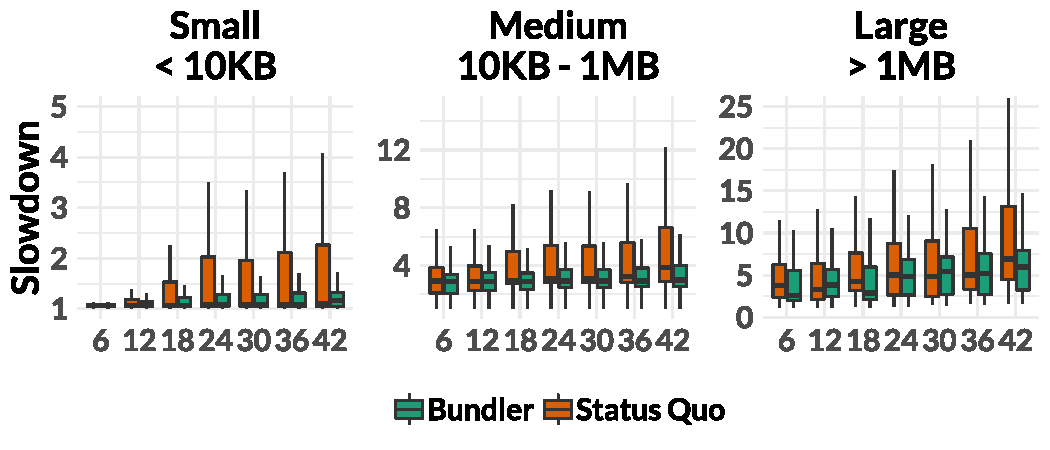
\includegraphics[width=\maxwidth]{figure/robust_cr-inelastic-1} 

\end{knitrout}
    \caption{Against cross traffic comprising of short lived flows. \name offers 48Mbps of load to the bottleneck queue. The cross traffic's offered load increases along the x-axis, while \name{}'s offered load remains fixed.}
    \label{fig:robust:cr-inelastic}
\end{figure}


We can see this phenomenon in action in Figure~\ref{fig:robust:cr-inelastic}.

\begin{outline}
\1 Use Copa-sfq and nimbus-sfq at 75\% or 87.5\% offered load, nobundler-fifo
\1 Cross traffic
\2 Inelastic cross traffic
\2 Elastic cross traffic

\1 Different RTTs
\1 Different bandwidths
\end{outline}
